%----------------------------------------------------------------------------
\chapter{Az end-to-end beszédfelismerés elmélete}
%----------------------------------------------------------------------------

\section{Hagyományostól az end-to-end-ig}

A hagyományos ASR-ok (automatikus beszédfelismerők) több elemből álló, összetett rendszerek, melyek manapság igen pontosan meg tudják állapítani mi volt az eredetileg elhangzott szöveg, és leképezik azt írásos formába. Az egyik legelterjedtebb a HMM (Rejtett Markov Modell) alapú beszédfelismerő rendszer [1]. A rendszernek több eleme is van: egy dekóder mely tartalmaz egy nyelv modellt, akusztikus modelleket és egy kiejtési szótárat is, illetve tartalmaz egy elemet, mely a bemeneti hangból a kiemeli jellemzőket, átalakítja őket a rendszer által kezelhető formájúvá. A HMM-en alapuló rendszerek fő eleme a Viterbi algoritmus \cite{viterbi}, mely dinamikus programozást alkalmazva találja meg a legjobb illeszkedést a bemeneti szöveg és az adott beszéd modell közt.

A rendszer különböző elemeo erősen függenek egymástól. Ha az egyik nem rendeltetés szerűén működik és rossz kimenetet ad, akár saját vagy egy korábbi elem hibájából kifolyólag az befolyásolja a többi elemet is, így elrontva, torzítva a kapott végeredményt. Az egyes elemeket külön-külön kell kalibrálni, tanítani és tökéletesíteni.

Ezzel szemben, a napjainkban egyre inkább népszerű, E2E (end-to-end) alapú beszédfelismerő rendszerek [2] sokkal egyszerűbb, kevesebb köztes elemet igénylő megközelítést nyújtanak. Bizonyos szituációkban, ahol egy specifikusabb szövegkörnyezetben, pl. pénzügyi vagy jogi, elhangzó szavak azonosítása a cél, már a hagyományos ASR rendszereknél is pontosabb eredményeket képesek produkálni.

Az E2E rendszerek mély neurális hálókon alapszanak, közvetlen bemenetük a nyers hang, kimenetük pedig a becsült szöveg. Természetesen a neurális háló bemenetéhez a hangot még előre fel kell dolgozni, amit pre-processing-nek neveznek. A háló kimenete pedig az egyes bemeneti időegységekre becsült karakterek valószínűségei melyekből ki kell nyerni a végső, feltételezett szöveget.

\section{A beszédfelismerés lépései}

\subsection{Előfeldolgozás}

A beszéd előfeldolgozása az első fontos lépése a beszédfelismerő rendszereknek. Vannak törekvések, melyekben a E2E neurális hálónak közvetlenül a nyers, feldolgozatlan hanganyagot adják meg és ez alapján tanítják [4], ezáltal még inkább tisztán a neurális háló működésére támaszkodva. Egyelőre ennek a megközelítésnek az eredményei messze elmaradnak a hang előfeldolgozásával elérhető SOTA modellek pontosságától.

A két fő megközelítés többnyire hasonló, apró eltérésekkel. Az egyik legelterjedtebb és bevált átalakítás a spektogram.

Ahogy az 1. ábrán is látható, a spektogramm három tengely mentén reprezentálja az adatot. A vízszintes tengelyen az idő, míg a függéleges tengelyen a frekvencia van megadva. Van továbbá egy harmadik tengely is, ami színnel van jelölve és mértékegysége a decibel. Ez a jel amplitúdója, ami az adott időpillanatban, adott frekvenciához tartozik és a szín intenzitása reprezentálja a kép pontjain mértékét.

A szokványos spektrogrammon kívül használatos még a MFCCs (Mel-Frequency Cepstral Coefficients) is. Felépítése hasonló a spektogramméval, viszont a frekvencia helyett MFC koefficiens \cite {mfcc} értéke van az y tengelyen. Ez a Mel skála, amely úgy van megválasztva, hogy a skálán egyelő távolságra lévő hangok az emberi fül számára is hasonló távolságúnak tűnjenek. A frekvenciához képest egy lényeges változást jelent, hiszen az ember számára könnyen hallható kisebb frekvenciákon, például az 500 Hz és 1000 Hz közötti különbség, míg 6500 Hz és 7000 Hz között már kevésbé számottevő az eltérés. Ez utóbbi érték nagyságrendekkel kisebb a frekvencia értéknél így lényegesen befolyásolhatja a neurális háló tanulási folyamatát.

Az előfeldolgozott jelet időegységekre bontjuk, melyek már a neurális háló bemenetét képzik. A kimeneten az egyes időegységekre kapott predikciókból pedig összeállítható a feltételezett szöveg.

\begin{figure}[!ht]
\centering
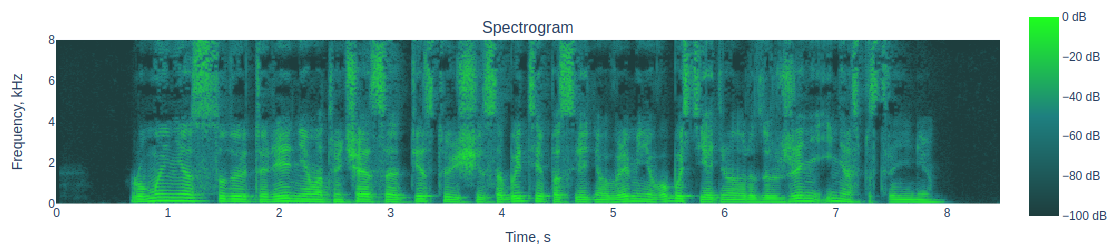
\includegraphics[width=150mm, keepaspectratio]{figures/spectogram.png}
\caption{Spectogram.}
\label{fig:TeXstudio}
\end{figure}

\subsection{Neurális hálók}

A neurális hálók az emberi idegek működésének mintája alapján modellezett láncolatok. Számos különböző, komplex feladat megoldására előszeretettel alkalmazzák őket. Röviden összefoglalva három fő alkotó részt kell elképzelni. Egyik a bemenet, például egy kép esetén a pixelek, beszédfelismerés esetén az egyes időpillanatokhoz tartozó értékek vektor formában. Spektogram esetén az időpillanathoz tartozó vektor egyes elemei a frekvenciát jelképezik és az elemek értéke pedig a hangerősséget.

A neurális háló közbülső, rejtettnek, nevezett része tetszőleges méreteket ölthet. Az egyes rétegek pontjai mindig az előző réteg pontjaival vannak összekötve úgy nevezett súlyok segítségével. Az újabb rétegek pontjainak értékét az abba befutó súlyok, illetve a súlyok és kiinduló pontjuk szorzatainak az összegével számítjuk. A pontok végső értéke még egy aktivációs függvénynek nevezett kiértékelésen is keresztül megy, mielőtt a következő réteg értékeit kiszámítatnánk vele. Az aktivációs függvények igen eltérőek lehetnek, egy népszerű függvény a ReLU, ami a 3.2-es ábrán látható. Ezeket a pontokat neuronoknak szokás nevezni, innen ered a neurálsi háló kifejezés. A háló tanítása során ezen súlyok értékét módosítjuk úgy, hogy a legoptimálisabb, számunkra kedvezőnek vélt eredményt kapjuk.

\begin{figure}[!ht]
\centering
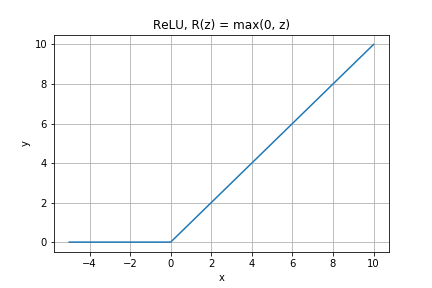
\includegraphics[width=125mm, keepaspectratio]{figures/ReLU.png}
\caption{A ReLU aktivációs függvény.}
\label{fig:TeXstudio}
\end{figure}

Az utolsó réteg a kimeneti réteg, ahol az eredményt kapjuk meg. A kimeneti réteg lehet regresszív, egy előre meg nem határozott, tetszőleges érték, vagy a mi esetünkben klasszifikáció, amikor előre meghatározott címkék (label-ek) valószínűségére vagyunk kíváncsiak. Legegyszerűbb estben a legvalószínűbb címke kerül kiválasztásra válaszként.

A valószínűség kiszámításához a softmax \cite{softmax} függvényt szokás használni, ami szintén egy aktivációs függvény. A függvény egy vektor bemenetet megkapva normalizálja a vektor egyes értékeit úgy, hogy azok új értékei 0 és 1 közé essenek, miközben az összegük pontosan 1-et adjon. A softmax függvény, ahol x a bemeneti vektort jelöli, míg i és j a vektor egyes elemeinek a sorszámát:

\begin{align}
softmax(x)_i = \frac{exp(x_i)}{\sum_{j}^{ }exp(x_j))}.
\end{align}

Neurális hálók egyik leggyakoribb tanítási módszere a felügyelt tanítás. Ez azt jelenti, hogy először például egy tanítatlan, véletlenszerűen inicializált, hálóból kiindulva kiértékeljük egy tetszőleges bemenetre a végeredményt. Majd a végeredmény helyességétől függően változtatjuk a súlyok értékét a hálóban: azon súlyokat melyek egy rossz eredmény nagyobb valószínűségéhez járultak hozzá büntetjük, csökkentjük az értéküket, míg azokat melyek egy jó eredmény pozitív értékéhez járultnak hozzá növeljük. Ezt a folyamatot szokás backpropagation-nak nevezni. A büntetés mértéke is létfontosságú, hiszen fontos, hogy ne csak az adott bemenetre tudjon pontos végeredményt adni a háló, hanem általánosan is pontos legyen. 

Az egyik legegyszerűbb réteg típus a Dense (sűrű) vagy más néven Fully Connected, ahogy a neve is utal rá az egyes neuronok a súlyokkal sűrűn vannak összekötve. Ez azt jelenti, hogy minden egyes réteg mindegyik neuronja össze van kötve az előző réteg összes neuronjával súlyokon keresztül. Több Dense réteg is követheti egymást, mely esetben az adott réteg összes neuronja össze van kötve a következő réteg összes neuronjával is.

Az E2E-hez használt leggyakoribb neurális háló réteg fajták az rekurrens (RNN) és konvolúciós (CNN) rétegek. Ez utóbbit elterjedten használják a különböző képfelismerő feladatok terültén is.

Lényegesen összetettebb a Dense rétegnél a konvolúciós réteg [5], melynél egy, a teljes bemenetnél kisebb, kernel-t (egyes forrásokban filter) mozgatunk végig a bemenet elemein és kiértékeljük az általa lefedett értékeket. A lefedett számokat a kernel velük fedésben lévő értékével összeszorozzuk, ezek az értékek főként a -1, 0 és 1, majd a kapott eredményeket összeadjuk. Ezt követően a kernel-t egy megadott értékkel, a stride-al mozgatva kiértékeljük a következő, kernel által lefedett számokat. A konvolúció végezhető egy vagy több dimenziós bemeneten, különböző kernel-ekkel párhuzamosan is, kép esetén például három csatornás képen, ahol a piros kék és zöld értékek külön csatornákon vannak reprezentálva. Egy opcionális lépés, hogy a bement széleit feltöltjük-e nullásokkal, ez az úgy nevezett zero padding. Ennek célja, hogy ugyan akkora legyen a kimenet, mint a padding nélküli bemenet volt. Ezen kívül is szükség lehet padding-re például egy 5x5-ös kép esetén, ha a kernel mérete 3x3 és a stride 3, akkor ki kell tölteni a kép széleit, hogy minden bemeneti értéken legalább egyszer végig menjen a kernel.

Egy CNN-hez kapcsolódó, kernellel rendelkező rétegtípus a pooling réteg, mely kifejezetten az adat méretének csökkenését szolgálja. Ezzel a célja a számítási kapacitás csökkentése, miközben minél inkább megőrzi az adatban rejlő információt. Két használt pooling típus a max vagy average pooling. Előbbinél a kernel által befoglalt értékek maximumát választja, míg utóbbinál az átlagukat.

A konvolúciós vagy pooling rétegek működésükből adódóan csökkenthetik a kimenetük méretét, ezáltal ismerni kell annak pontos dimenzióját, a következő réteghez kapcsolódó számítások végett. A kimenet méretét a következő képlettel lehet kiszámolni, ahol ’O’ a kimenet mérete, ’W’ a bemenet mérete, ’P’ a padding mérete, ’K’ a kernel mérete és ’S’ a stride:

\begin{align}
\mathbf{O}&=\frac{\mathbf{W}-\mathbf{K}+\mathbf{2P}}{\mathbf{S}+\mathbf(1)}.
\end{align}

A rekurrens rétegek [6] egyik legérdekesebb tulajdonsága, hogy nem csupán a bemeneti súlyaikat használják a neuronok kiértékeléséhez, így felhasználva a korábban tanultakat, hanem emlékeznek a korábbi neuron értékeikre is, melyek szintén befolyásolják az aktuális bemenetre kapott eredményt. Beszédfelismerés esetén ezt úgy is el lehet képzelni, hogy ha például elhangzik egy magánhangzó, akkor utána nagy valószínűséggel egy mássalhangzót várunk, ennek fényében, sikeres tanítás esetén, a mássalhangzókat részesíti előnyben egy azt megelőző magánhangzó után. Korábbi időpillanatok, állapotok tehát hozzájárulnak egy újabb állapot kiértékeléséhez a rekurrens rétegben, ahogy ez a 3.3-as ábrán is látható.
 
\begin{figure}[!ht]
\centering
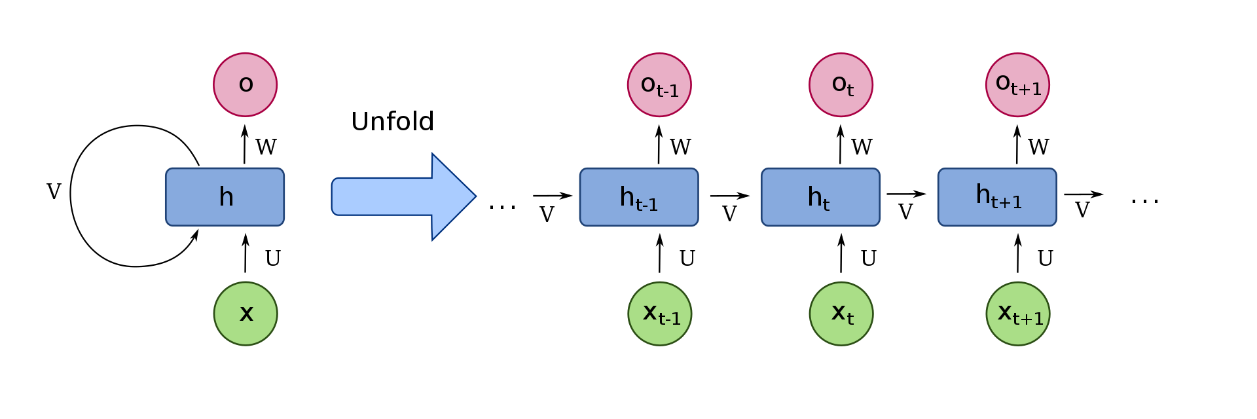
\includegraphics[width=150mm, keepaspectratio]{figures/rnn.png}
\caption{A rekurrens réteg "kigörgetve" \cite{rnn}.}
\label{fig:TeXstudio}
\end{figure}

Két altípusa a rekurrens hálóknak az LSTM és GRU (Long Short Term Memory, Gated Recurrent Unit). Ezek a típusok hasonló elveken működnek, a különbség a neuronok korábbi értékeinek újabb értékekre történő ráhatásának számítási módjában rejlik. Az LSTM [7] fő célja, hogy kijátssza a hagyományos rekurrens hálók egyik legnagyobb problémáját, azt, hogy a régebbi bemenet súlya nincs hasonló fontossággal kezelve, mint a jelenlegi bemenethez közelebbi érték. Könnyen belátható, hogy fontos lehet egy mondat végi szót vizsgálva, hogy mi volt a szó a mondat elején, akár a vizsgálandó mondat elemet megelőző néhány szónál is. Az LSTM kapukat használ annak megelőzése céljából, hogy egy korábbi értékelés elvesszen, ezáltal kezelhetetlenné téve annak beleszámítását az újabb értékelésnél.

A GRU egy LSTM-hez hasonló újabb fejlesztésű réteg. Egyik fő tulajdonsága, hogy kevesebb elemet tartalmaz, így kevesebb paramétert használ, csökkentve a neurális háló komplexitását, ezáltal a szükséges számítási időt is.

Megemlítendő még a Bi-directional (két irányú) réteg, amely mögött az a gondolat húzódik meg, hogy ne csak a múltbéli bemenetek befolyásolják az adott bemenetünket, hanem a jövőbeliek is. Két rekurrens réteget használ, melyek ellentétes irányban haladnak egymással, így tetszőleges kiértékelésnél használhatóak a korábbi, illetve elkövetkezendő neuronok eredményei is.

\subsection{CTC dekódolás és loss számítás}

A CTC (Connectionist Temporal Classification) \cite{ctc} funkciója a kimeneti dekódolása, a válasz kiértékelése, mely folyamán átalakítja a kimenetet a megadott címkék valószínűségi szekvenciájára. A címkék lehetnek az egyes karakterek, amik egy adott nyelvben előfordulhatnak. Ez esetben a CTC kiértékeli, hogy melyik betű vagy egyéb karakter hangzott el adott időpillanatban, adott bemenetre [8]. Ereje abban rejlik, hogy nincs szükség a kiértékelésnél a kimeneteket egyenként, karakter szinten összekötni az elvárt szöveggel, elegendő a kimeneti szöveget megadni, azt, amit kapni szeretnék az adott bemenetre. Másik fontos előnye, hogy a felismert szöveget nem szükséges külön feldolgozni, mivel átalakítja azt a végleges, feltételezett formára. Feldolgozza, hogy egy hosszú hang esetén, mint az ’ú’ több időpillanaton keresztül is hallatszik az ’ú’ betű, de nekünk a végeredményben csak egy darab ’ú’ szükséges.

Felmerülhet egy probléma az összevonással, amikor olyan egymást követő betűket vonunk össze, melyek a szóban külön szerepelnek, mint például az ’ellentét’ szóban. Ennek elkerülése végett bevezet a CTC egy üres karaktert, ami nem egyenlő a szóközzel, és ezt olyan időegységekhez helyezi, ahol nem ismerhető fel betű a megadott szótárból, karaktergyűjteményből. Az ilyen üres karakterrel elválasztott betűket nem fogja összevonni kiértékeléskor.

A neurális háló által végzett kiértékelés után az ember által feldolgozható kimenet megszerzéséig szükség van még a karakterek összeillesztésére. Ehhez különböző elven működő dekódolókat használunk. Az egyik legalapvetőbb dekódolási algoritmus a best path eljárás. Két dolgot végez: kiszámolja a legvalószínűbb útvonalat a kapott kimeneti időegységeken át, majd eltávolítja az egymást követő azonos karaktereket, melyek közt nem található az üres karakter. Végül az üres karaktereket is eltávolítja, így eredményezve a végső predikciót.

További feladata a neurális háló tanításához használt loss kiszámítása \cite{ctc_sid}. A hiba számítása során a szempontunkból lényegtelen milyen karaktersorozattal jut el a végeredményhez, csupán az a cél, hogy pontosan az adott kimenetet eredményezze. A loss-t tehát úgy számítja, hogy megnézi az összes olyan karaktersorozat valószínűségét, melyből megkaphatja a kívánt eredményt és összegzi őket. Ezáltal az eredeti GT (Ground Truth) szöveg valószínűségi értéke magas, hogyha a megszerzéséhez szükséges kombinációk értékének az összege magas.

A CTC loss számítása a 3.3-as, 3.4-es és 3.5-ös képeltek alapján történik, ahol GT az elvárt szöveg, X az egyes akusztikus keretek, C egy adott karaktersorozat és $c_t$ egy adott karakter adott időpillanatban.
\begin{align}
CTC loss&=-\log{P(GT | X)}.
\end{align}

Összes lehetséges helyes karaktersorozat valószínűségének az összege:
\begin{align}
P(GT | X)&=\sum_{C=A(GT)} P(C | X).
\end{align}

Egy adott, helyes karaktersorozat valószínűsége:
\begin{align}
P(C | X)&=\prod_{t=1}^{T} y(c_t, t)).
\end{align}

\section{Létező megoldások}

A beszédfelismerő rendszereket pontosságuk alapján tudjuk rangsorolni. Egy nemzetközileg elismert pontossági mérőszám a WER (Word Error Rate). Ezt a pontosságot szokás szerint egy publikusan elérhető, angol nyelvű hangoskönyv felolvasásokat tartalmazó adatbázison, a LibriSpeech-en\footnote{LibriSpeech oldala: \url{http://www.openslr.org/12/}} mérik.

Különböző, alacsony hibaarányú modellek léteznek, de ez egyik lekiemelkedőbb közülök az Nvidia QuartzNet\footnote{Az Nvidia ismertető oldala: \url{https://developer.nvidia.com/blog/develop-smaller-speech-recognition-models-with-nvidias-nemo-framework/}} modellje, mely alacsony számú paraméterek mellett képes igen nagy precíziót fenntartani. Míg a QuartzNet bonyolultsága, paramétereinek a száma csupán töredéke a legtöbb SOTA modellének, a WER száma megközelíti azokét (3.1-es táblázat).

A modellekben elterjedt a konvolúciós- (CNN) és rekurrens neurális rétegek  (RNN) használata.

\begin{table}[ht]
	\footnotesize
	\centering
	\begin{tabular}{ p{2cm} p{2.5cm} p{2.5cm} p{1.5cm} p{1.5cm} p{1.5cm} }
		\toprule
		\textbf{Model} & \textbf{Aug} & \textbf{LM} & \textbf{clean WER(\%)} & \textbf{other WER(\%)} & \textbf{Million Parameters} \\
		\midrule
		wav2letter++ & Speed Perturb & ConvLM & 3.26 & 10.47 & 208 \\
		\hline
		LAS & SpecAugment & RNN & 2.5 & 5.8 & 360 \\
		\hline
		Time-Depth Separable Convolutions & Dropout, Label Smoothing & N/A (greedy) & 5.36 & 15.64 & 37 \\
		&  & 4-gram & 4.21 & 11.87 &  \\
		&  & ConvLM & 3.28 & 9.84 &  \\
		\hline
		Multi-Stream Self-Attention & Speed Perturb & 4-gram & 2.93 & 8.32 & 23  \\
		&  & 4-LSTM & 2.20 & 5.82 &  \\
		\hline
		QuartzNet-15x5 & Spec Cutout, Speed Perturb & N/A (greedy) & 3.90 & 11.28 & 19 \\
		&  & 6-gram & 2.96 & 8.07 &  \\
		&  & Transformer-XL & 2.69 & 7.25 &  \\
		\bottomrule
	\end{tabular}
	\caption{Egyes angol nyelven tanult SOTA beszédfelismerő modellek és paramétereik.}
\end{table}

\section{Következtetések}

Megoldásomban az Nvidia QuartzNet alapján indultam el, annak alacsony paraméterszámát figyelembe véve. Egy Pytorch alapú toolkit-et, az Nvidia NeMo-t (Neural Modules) használva kísérleteztem QuartzNet kombinációkkal.

Főként az ingyenesen hozzáférhető Mozilla Common Voice adatbázist használva tanítottam orosz nyelvre a legsikeresebbnek ítélt, 15x5 architektúrájú modellt. A modellt nem véletlenszerűen beállított súlyokkal, hanem transfer learning-et alkalmazva, egy előre tanított angol modellbeli súlyokkal inicializáltam.

Az eredmény finomítása végett próbálkoztam több tanítóadat beiktatásával, mellyel a validációs adathalmaz WER értéke csökkent, így javult. Sajnos a több tanítóadat lényeges megnövelte a tanítás idejét így erőforrások szűkében csökkentette a kísérletezésre jutó időt, ezért ezt a módszert csak kis mértékben alkalmaztam.
